\section{Opgave 1 - Process statements}
\begin{enumerate}
	\item[1)]
	Vi skriver behavioral style koden som vist i figur \ref{lst:processState}
		
		\begin{lstlisting}[caption={Behavioral style kode for en AND og OR gate},label={lst:processState}]
		library ieee;
		use ieee.std_logic_1164.all;
		
		entity process_statement is 
		port (a, b, c : in std_logic;
		f : out std_logic);
		end process_statement;
		
		architecture two_processes of process_statement is
		signal i1 : std_logic;
		begin
		u1: process (a, b)
		begin
		i1<=a and b;
		end process u1;
		
		u2: process (i1, c)
		begin
		f<=i1 or c;
		end process u2;
		
		end two_processes;
		\end{lstlisting}
		Med RTL-vieweren på figur \ref{fig:RTL process}  kan vi se at vores kode stemmer overens med det system vi har skrevet koden efter.
		\begin{figure}[h]
			\centering
			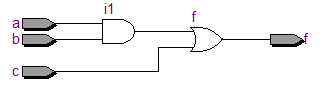
\includegraphics[scale=0.8]{pictures/Oevelse5/opg1/RTL_process.JPG}
			\caption{}
			\label{fig:RTL process}
		\end{figure}
		\item[2)]
		\begin{figure}[h]
			\centering
			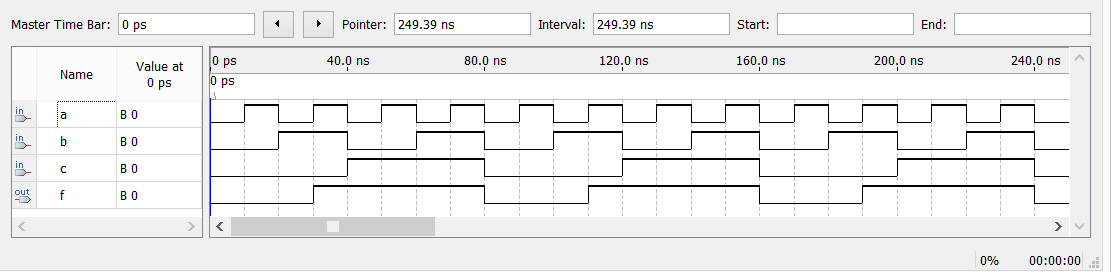
\includegraphics[scale=0.8]{pictures/Oevelse5/opg1/func_sim_process.JPG}
			\caption{}
			\label{fig:Functional simulation process koden}
		\end{figure}
	\item[3)]
	Vi skriver koden for truth-tabellen sådan at x og y bliver initialiseret i hver deres proces, som det ses i figur \ref{lst:truthtab} 
	\begin{lstlisting}[caption={Behavioral style kode for truth tabellen},label={lst:truthtab}]
	library ieee;
	use ieee.std_logic_1164.all;
	
	entity process_statement2 is 
	port (a, b, c : in std_logic;
	x, y : out std_logic);
	end process_statement2;
	
	architecture xy_processes of process_statement2 is
	signal i1 : std_logic_vector(2 downto 0);
	begin
	i1 <= a&b&c;
	u1: process (i1)
	begin
	if i1 = "000" then x <= '0';
	elsif i1 = "001" then x <= '1';
	elsif i1 = "010" then x <= '0';
	elsif i1 = "011" then x <= '0';
	elsif i1 = "100" then x <= '1';
	elsif i1 = "101" then x <= '0';
	elsif i1 = "110" then x <= '0';
	elsif i1 = "111" then x <= '0';
	end if;
	end process u1;
	
	u2: process (i1)
	begin
	if i1 = "000" then y <= '1';
	elsif i1 = "001" then y <= '0';
	elsif i1 = "010" then y <= '1';
	elsif i1 = "011" then y <= '0';
	elsif i1 = "100" then y <= '0';
	elsif i1 = "101" then y <= '0';
	elsif i1 = "110" then y <= '0';
	elsif i1 = "111" then y <= '1';
	end if;
	end process u2;
	
	end xy_processes;
	\end{lstlisting}
	\begin{figure}[h]
		\centering
		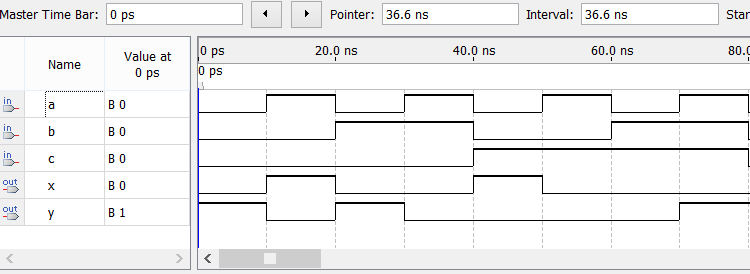
\includegraphics[scale=0.75]{pictures/Oevelse5/opg1/func_sim_truth.JPG}
		\caption{}
		\label{fig:Functional simulation af Truth tabel.}
	\end{figure}
\end{enumerate}